\documentclass{article}%
\usepackage[T1]{fontenc}%
\usepackage[utf8]{inputenc}%
\usepackage{lmodern}%
\usepackage{textcomp}%
\usepackage{lastpage}%
\usepackage[tmargin=1cm,bmargin=2cm,lmargin=1cm]{geometry}%
\usepackage{multicol}%
\usepackage{graphicx}%
\usepackage{adjustbox}%
\usepackage{tkz-euclide}%
\usepackage{amsmath}%
\usepackage{scalefnt}%
\usepackage{enumitem}%
%
%
%
\begin{document}%
\normalsize%
\setlength\itemsep{-2cm}%
\section{January 14: Linear Equations and Slope Review}%
\label{sec:January14LinearEquationsandSlopeReview}%
\textbf{Learning Goal: }\hrulefill \\ \hrulefill%
\begin{multicols}{2}%
\begin{enumerate}[label=\arabic*),start=1]%
\item\adjustbox{valign=t}{\begin{minipage}{\linewidth}
Graph the equation $y=2/5x+2$.\\

%\vspace{4cm}

\begin{tikzpicture}[font=\small,scale=0.40]
   \tikzstyle{every node}=[font=\small]
   \tkzInit[xmax=6,ymax=6,xmin=-6,ymin=-6]
   \tkzGrid
   \tkzAxeXY
%   \draw[ thick,latex-latex] (-1,4) -- (4,-6) node[anchor=south west] {$a$}; % two points for drawing 2x+y=2
%  \tkzText[above](0,6.75){Desired Output}
  \end{tikzpicture}
\end{minipage}}%
\vspace{0cm}%
\item\adjustbox{valign=t}{\begin{minipage}{\linewidth}
Graph the equation $y=-2x+4$.\\

%\vspace{4cm}

\begin{tikzpicture}[font=\small,scale=0.40]
   \tikzstyle{every node}=[font=\small]
   \tkzInit[xmax=6,ymax=6,xmin=-6,ymin=-6]
   \tkzGrid
   \tkzAxeXY
%   \draw[ thick,latex-latex] (-1,4) -- (4,-6) node[anchor=south west] {$a$}; % two points for drawing 2x+y=2
%  \tkzText[above](0,6.75){Desired Output}
  \end{tikzpicture}
\end{minipage}}%
\vspace{0cm}%
\item\adjustbox{valign=t}{\begin{minipage}{\linewidth}
Graph the equation $y = 6x-9$.\\

%\vspace{4cm}

\begin{tikzpicture}[font=\small,scale=0.40]
   \tikzstyle{every node}=[font=\small]
   \tkzInit[xmax=6,ymax=6,xmin=-6,ymin=-6]
   \tkzGrid
   \tkzAxeXY
%   \draw[ thick,latex-latex] (-1,4) -- (4,-6) node[anchor=south west] {$a$}; % two points for drawing 2x+y=2
%  \tkzText[above](0,6.75){Desired Output}
  \end{tikzpicture}
\end{minipage}}%
\vspace{0cm}%
\item\adjustbox{valign=t}{\begin{minipage}{\linewidth}
Graph the equation $y=-x+5$.\\

%\vspace{4cm}

\begin{tikzpicture}[font=\small,scale=0.40]
   \tikzstyle{every node}=[font=\small]
   \tkzInit[xmax=6,ymax=6,xmin=-6,ymin=-6]
   \tkzGrid
   \tkzAxeXY
%   \draw[ thick,latex-latex] (-1,4) -- (4,-6) node[anchor=south west] {$a$}; % two points for drawing 2x+y=2
%  \tkzText[above](0,6.75){Desired Output}
  \end{tikzpicture}
\end{minipage}}%
\vspace{0cm}%
\item\adjustbox{valign=t}{\begin{minipage}{\linewidth}
Graph the equation $y = 5/2x-5$.\\

%\vspace{4cm}

\begin{tikzpicture}[font=\small,scale=0.40]
   \tikzstyle{every node}=[font=\small]
   \tkzInit[xmax=6,ymax=6,xmin=-6,ymin=-6]
   \tkzGrid
   \tkzAxeXY
%   \draw[ thick,latex-latex] (-1,4) -- (4,-6) node[anchor=south west] {$a$}; % two points for drawing 2x+y=2
%  \tkzText[above](0,6.75){Desired Output}
  \end{tikzpicture}
\end{minipage}}%
\vspace{0cm}%
\item\adjustbox{valign=t}{\begin{minipage}{\linewidth}
Graph the equation $y=-1/2x+2$.\\

%\vspace{4cm}

\begin{tikzpicture}[font=\small,scale=0.40]
   \tikzstyle{every node}=[font=\small]
   \tkzInit[xmax=6,ymax=6,xmin=-6,ymin=-6]
   \tkzGrid
   \tkzAxeXY
%   \draw[ thick,latex-latex] (-1,4) -- (4,-6) node[anchor=south west] {$a$}; % two points for drawing 2x+y=2
%  \tkzText[above](0,6.75){Desired Output}
  \end{tikzpicture}
\end{minipage}}%
\vspace{0cm}%
\item\adjustbox{valign=t}{\begin{minipage}{\linewidth}
Graph the equation $y=1/2x+6$.\\

%\vspace{4cm}

\begin{tikzpicture}[font=\small,scale=0.40]
   \tikzstyle{every node}=[font=\small]
   \tkzInit[xmax=6,ymax=6,xmin=-6,ymin=-6]
   \tkzGrid
   \tkzAxeXY
%   \draw[ thick,latex-latex] (-1,4) -- (4,-6) node[anchor=south west] {$a$}; % two points for drawing 2x+y=2
%  \tkzText[above](0,6.75){Desired Output}
  \end{tikzpicture}
\end{minipage}}%
\vspace{0cm}%
\item\adjustbox{valign=t}{\begin{minipage}{\linewidth}
Graph the equation $y = -x-5$.\\

%\vspace{4cm}

\begin{tikzpicture}[font=\small,scale=0.40]
   \tikzstyle{every node}=[font=\small]
   \tkzInit[xmax=6,ymax=6,xmin=-6,ymin=-6]
   \tkzGrid
   \tkzAxeXY
%   \draw[ thick,latex-latex] (-1,4) -- (4,-6) node[anchor=south west] {$a$}; % two points for drawing 2x+y=2
%  \tkzText[above](0,6.75){Desired Output}
  \end{tikzpicture}
\end{minipage}}%
\vspace{0cm}%
\item\adjustbox{valign=t}{\begin{minipage}{\linewidth}
What is the slope of the graph below?\\

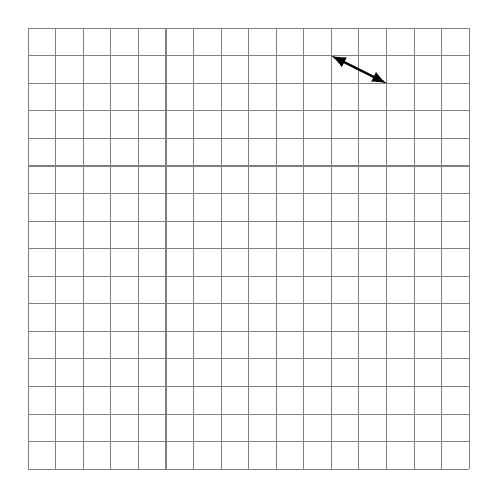
\begin{tikzpicture}[font=\tiny,scale=0.35]
   %\tikzstyle{every node}=[font=\small]
   \tkzInit[xmax=8,ymax=8,xmin=-8,ymin=-8]
   \tkzGrid
   \tkzAxeXY
   \draw[ thick,latex-latex] (5,6) -- (3,7);% node[anchor=south west] {$a$}; % two points for drawing 2x+y=2
%  \tkzText[above](0,6.75){Desired Output}
  \end{tikzpicture}
\end{minipage}}%
\vspace{0cm}%
\item\adjustbox{valign=t}{\begin{minipage}{\linewidth}
What is the slope of the graph below?\\

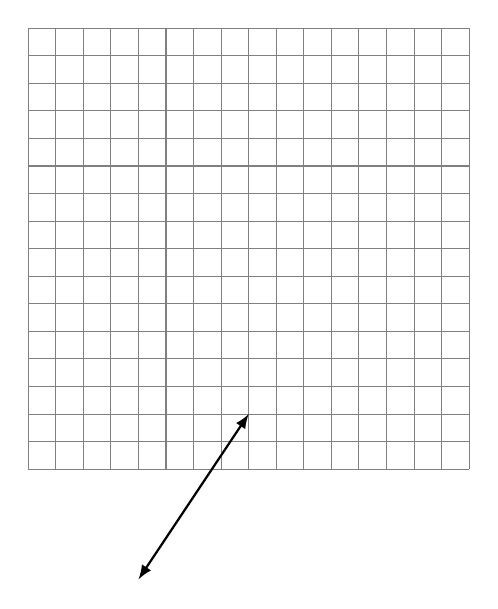
\begin{tikzpicture}[font=\tiny,scale=0.35]
   %\tikzstyle{every node}=[font=\small]
   \tkzInit[xmax=8,ymax=8,xmin=-8,ymin=-8]
   \tkzGrid
   \tkzAxeXY
   \draw[ thick,latex-latex] (0,-6) -- (-4,-12);% node[anchor=south west] {$a$}; % two points for drawing 2x+y=2
%  \tkzText[above](0,6.75){Desired Output}
  \end{tikzpicture}
\end{minipage}}%
\vspace{0cm}%
\item\adjustbox{valign=t}{\begin{minipage}{\linewidth}
What is the slope of the graph below?\\

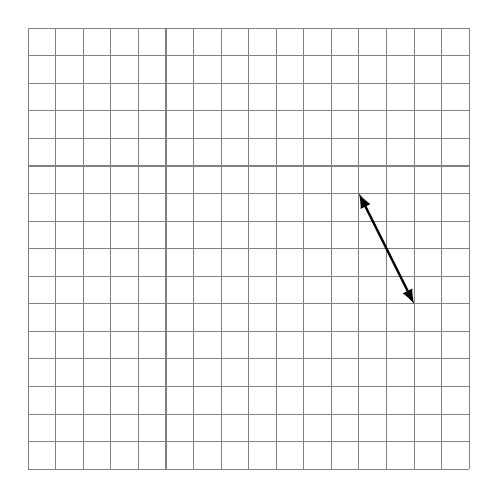
\begin{tikzpicture}[font=\tiny,scale=0.35]
   %\tikzstyle{every node}=[font=\small]
   \tkzInit[xmax=8,ymax=8,xmin=-8,ymin=-8]
   \tkzGrid
   \tkzAxeXY
   \draw[ thick,latex-latex] (4,2) -- (6,-2);% node[anchor=south west] {$a$}; % two points for drawing 2x+y=2
%  \tkzText[above](0,6.75){Desired Output}
  \end{tikzpicture}
\end{minipage}}%
\vspace{0cm}%
\item\adjustbox{valign=t}{\begin{minipage}{\linewidth}
What is the slope of the graph below?\\

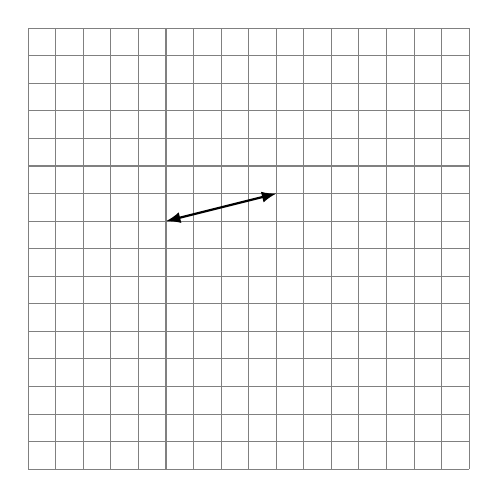
\begin{tikzpicture}[font=\tiny,scale=0.35]
   %\tikzstyle{every node}=[font=\small]
   \tkzInit[xmax=8,ymax=8,xmin=-8,ymin=-8]
   \tkzGrid
   \tkzAxeXY
   \draw[ thick,latex-latex] (1,2) -- (-3,1);% node[anchor=south west] {$a$}; % two points for drawing 2x+y=2
%  \tkzText[above](0,6.75){Desired Output}
  \end{tikzpicture}
\end{minipage}}%
\vspace{0cm}%
\item\adjustbox{valign=t}{\begin{minipage}{\linewidth}
What is the slope of the graph below?\\

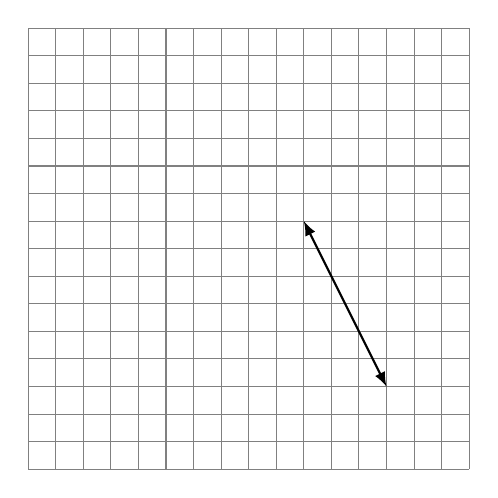
\begin{tikzpicture}[font=\tiny,scale=0.35]
   %\tikzstyle{every node}=[font=\small]
   \tkzInit[xmax=8,ymax=8,xmin=-8,ymin=-8]
   \tkzGrid
   \tkzAxeXY
   \draw[ thick,latex-latex] (5,-5) -- (2,1);% node[anchor=south west] {$a$}; % two points for drawing 2x+y=2
%  \tkzText[above](0,6.75){Desired Output}
  \end{tikzpicture}
\end{minipage}}%
\vspace{0cm}%
\item\adjustbox{valign=t}{\begin{minipage}{\linewidth}
What is the slope of the graph below?\\

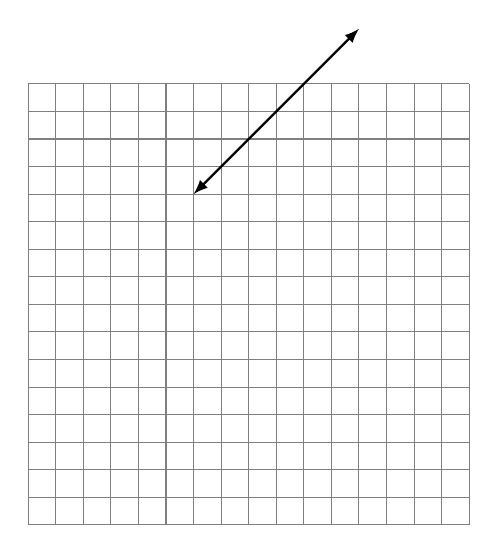
\begin{tikzpicture}[font=\tiny,scale=0.35]
   %\tikzstyle{every node}=[font=\small]
   \tkzInit[xmax=8,ymax=8,xmin=-8,ymin=-8]
   \tkzGrid
   \tkzAxeXY
   \draw[ thick,latex-latex] (-2,4) -- (4,10);% node[anchor=south west] {$a$}; % two points for drawing 2x+y=2
%  \tkzText[above](0,6.75){Desired Output}
  \end{tikzpicture}
\end{minipage}}%
\vspace{0cm}%
\item\adjustbox{valign=t}{\begin{minipage}{\linewidth}
What is the slope of the graph below?\\

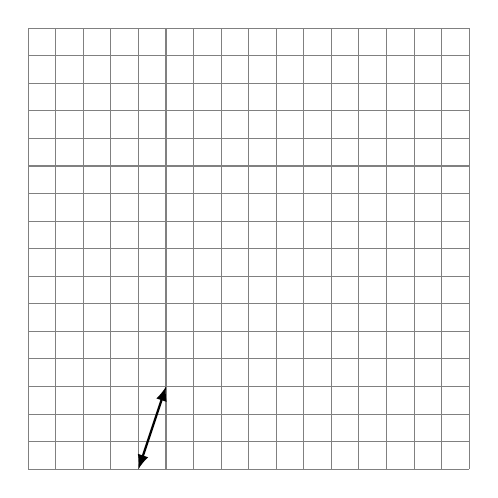
\begin{tikzpicture}[font=\tiny,scale=0.35]
   %\tikzstyle{every node}=[font=\small]
   \tkzInit[xmax=8,ymax=8,xmin=-8,ymin=-8]
   \tkzGrid
   \tkzAxeXY
   \draw[ thick,latex-latex] (-3,-5) -- (-4,-8);% node[anchor=south west] {$a$}; % two points for drawing 2x+y=2
%  \tkzText[above](0,6.75){Desired Output}
  \end{tikzpicture}
\end{minipage}}%
\vspace{0cm}%
\item\adjustbox{valign=t}{\begin{minipage}{\linewidth}
What is the slope of the graph below?\\

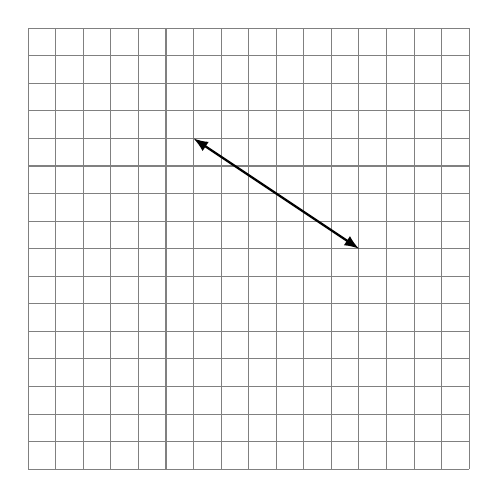
\begin{tikzpicture}[font=\tiny,scale=0.35]
   %\tikzstyle{every node}=[font=\small]
   \tkzInit[xmax=8,ymax=8,xmin=-8,ymin=-8]
   \tkzGrid
   \tkzAxeXY
   \draw[ thick,latex-latex] (-2,4) -- (4,0);% node[anchor=south west] {$a$}; % two points for drawing 2x+y=2
%  \tkzText[above](0,6.75){Desired Output}
  \end{tikzpicture}
\end{minipage}}%
\vspace{0cm}%
\item\adjustbox{valign=t}{\begin{minipage}{\linewidth}
What is the slope of the graph below?\\

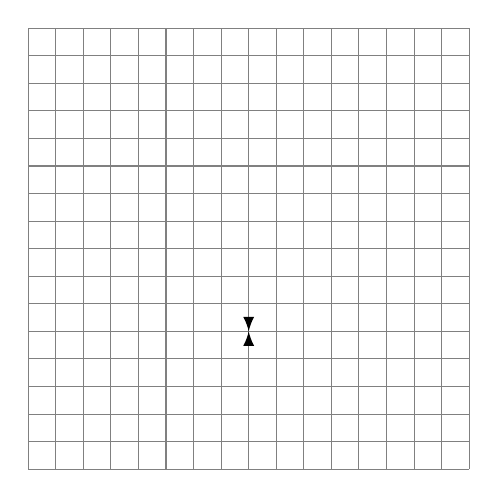
\begin{tikzpicture}[font=\tiny,scale=0.35]
   %\tikzstyle{every node}=[font=\small]
   \tkzInit[xmax=8,ymax=8,xmin=-8,ymin=-8]
   \tkzGrid
   \tkzAxeXY
   \draw[ thick,latex-latex] (0,-3) -- (0,-3);% node[anchor=south west] {$a$}; % two points for drawing 2x+y=2
%  \tkzText[above](0,6.75){Desired Output}
  \end{tikzpicture}
\end{minipage}}%
\vspace{1.75cm}%
\item\adjustbox{valign=t}{\begin{minipage}{\linewidth}
What is the slope of the graph below?\\

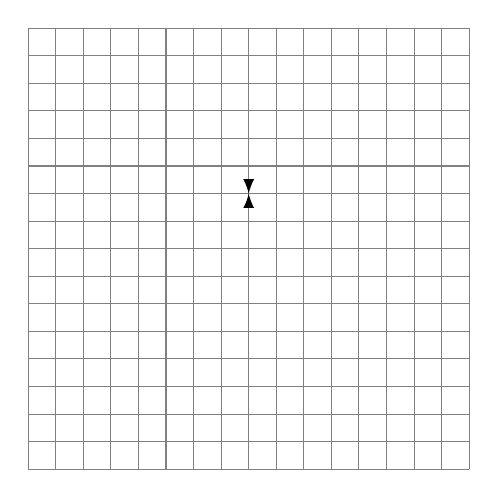
\begin{tikzpicture}[font=\tiny,scale=0.35]
   %\tikzstyle{every node}=[font=\small]
   \tkzInit[xmax=8,ymax=8,xmin=-8,ymin=-8]
   \tkzGrid
   \tkzAxeXY
   \draw[ thick,latex-latex] (0,2) -- (0,2);% node[anchor=south west] {$a$}; % two points for drawing 2x+y=2
%  \tkzText[above](0,6.75){Desired Output}
  \end{tikzpicture}
\end{minipage}}%
\vspace{1.75cm}%
\item\adjustbox{valign=t}{\begin{minipage}{\linewidth}
What is the slope of the graph below?\\

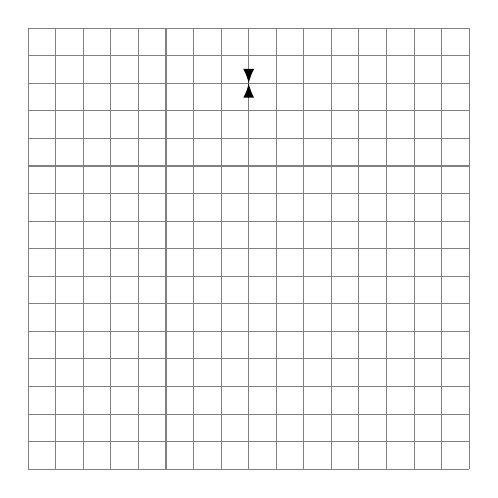
\begin{tikzpicture}[font=\tiny,scale=0.35]
   %\tikzstyle{every node}=[font=\small]
   \tkzInit[xmax=8,ymax=8,xmin=-8,ymin=-8]
   \tkzGrid
   \tkzAxeXY
   \draw[ thick,latex-latex] (0,6) -- (0,6);% node[anchor=south west] {$a$}; % two points for drawing 2x+y=2
%  \tkzText[above](0,6.75){Desired Output}
  \end{tikzpicture}
\end{minipage}}%
\vspace{1.75cm}%
\item\adjustbox{valign=t}{\begin{minipage}{\linewidth}
What is the slope of the graph below?\\

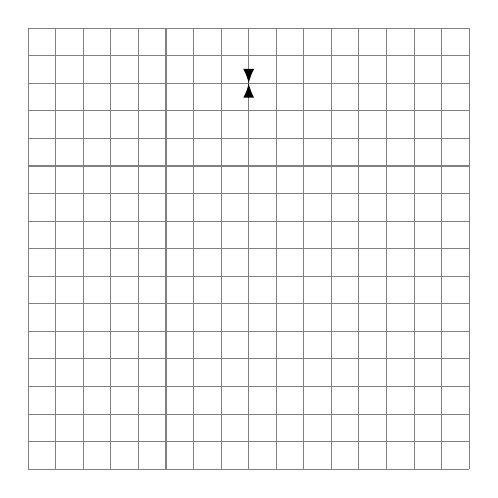
\begin{tikzpicture}[font=\tiny,scale=0.35]
   %\tikzstyle{every node}=[font=\small]
   \tkzInit[xmax=8,ymax=8,xmin=-8,ymin=-8]
   \tkzGrid
   \tkzAxeXY
   \draw[ thick,latex-latex] (0,6) -- (0,6);% node[anchor=south west] {$a$}; % two points for drawing 2x+y=2
%  \tkzText[above](0,6.75){Desired Output}
  \end{tikzpicture}
\end{minipage}}%
\vspace{1.75cm}%
\item\adjustbox{valign=t}{\begin{minipage}{\linewidth}
What is the slope of the graph below?\\

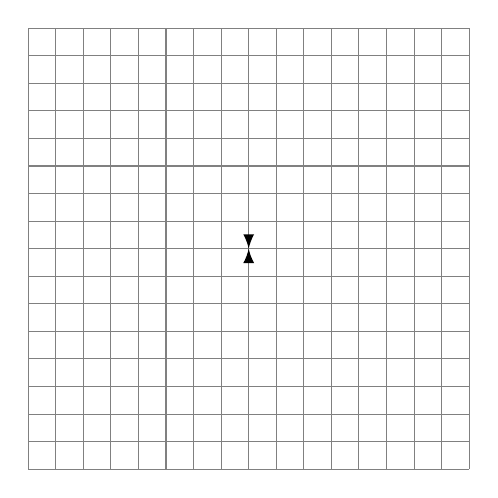
\begin{tikzpicture}[font=\tiny,scale=0.35]
   %\tikzstyle{every node}=[font=\small]
   \tkzInit[xmax=8,ymax=8,xmin=-8,ymin=-8]
   \tkzGrid
   \tkzAxeXY
   \draw[ thick,latex-latex] (0,0) -- (0,0);% node[anchor=south west] {$a$}; % two points for drawing 2x+y=2
%  \tkzText[above](0,6.75){Desired Output}
  \end{tikzpicture}
\end{minipage}}%
\vspace{1.75cm}%
\item\adjustbox{valign=t}{\begin{minipage}{\linewidth}
What is the slope of the graph below?\\

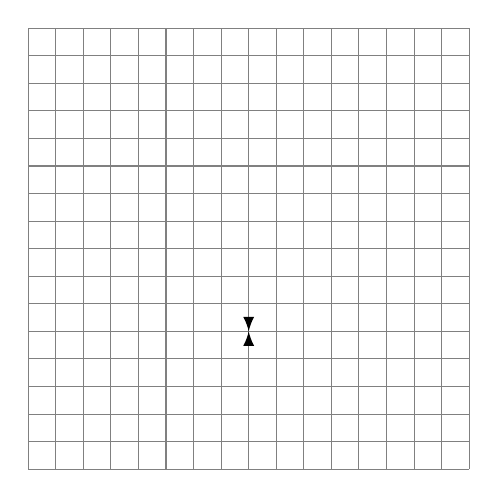
\begin{tikzpicture}[font=\tiny,scale=0.35]
   %\tikzstyle{every node}=[font=\small]
   \tkzInit[xmax=8,ymax=8,xmin=-8,ymin=-8]
   \tkzGrid
   \tkzAxeXY
   \draw[ thick,latex-latex] (0,-3) -- (0,-3);% node[anchor=south west] {$a$}; % two points for drawing 2x+y=2
%  \tkzText[above](0,6.75){Desired Output}
  \end{tikzpicture}
\end{minipage}}%
\vspace{1.75cm}%
\item\adjustbox{valign=t}{\begin{minipage}{\linewidth}
What is the slope of the graph below?\\

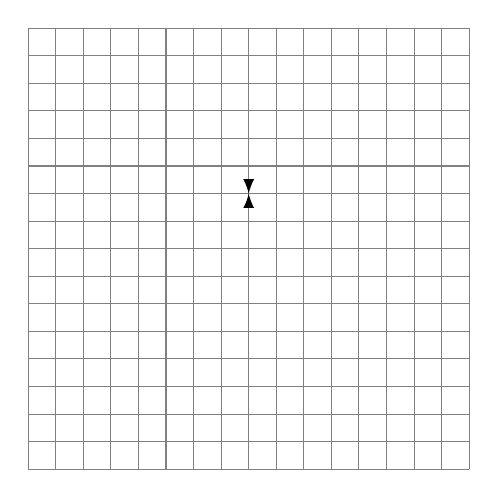
\begin{tikzpicture}[font=\tiny,scale=0.35]
   %\tikzstyle{every node}=[font=\small]
   \tkzInit[xmax=8,ymax=8,xmin=-8,ymin=-8]
   \tkzGrid
   \tkzAxeXY
   \draw[ thick,latex-latex] (0,2) -- (0,2);% node[anchor=south west] {$a$}; % two points for drawing 2x+y=2
%  \tkzText[above](0,6.75){Desired Output}
  \end{tikzpicture}
\end{minipage}}%
\vspace{1.75cm}%
\item\adjustbox{valign=t}{\begin{minipage}{\linewidth}
What is the slope of the graph below?\\

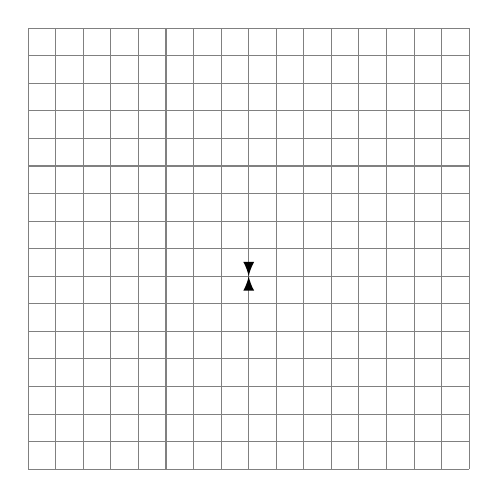
\begin{tikzpicture}[font=\tiny,scale=0.35]
   %\tikzstyle{every node}=[font=\small]
   \tkzInit[xmax=8,ymax=8,xmin=-8,ymin=-8]
   \tkzGrid
   \tkzAxeXY
   \draw[ thick,latex-latex] (0,-1) -- (0,-1);% node[anchor=south west] {$a$}; % two points for drawing 2x+y=2
%  \tkzText[above](0,6.75){Desired Output}
  \end{tikzpicture}
\end{minipage}}%
\vspace{1.75cm}%
\item\adjustbox{valign=t}{\begin{minipage}{\linewidth}
Find the slope of the line through $(-4,-2)$ and $(-4,-1)$.\\

\end{minipage}}%
\vspace{1.75cm}%
\item\adjustbox{valign=t}{\begin{minipage}{\linewidth}
Find the slope of the line through $(3,0)$ and $(2,-2)$.\\

\end{minipage}}%
\vspace{1.75cm}%
\item\adjustbox{valign=t}{\begin{minipage}{\linewidth}
Find the slope of the line through $(2,4)$ and $(-2,2)$.\\

\end{minipage}}%
\vspace{1.75cm}%
\item\adjustbox{valign=t}{\begin{minipage}{\linewidth}
Find the slope of the line through $(3,0)$ and $(-2,3)$.\\

\end{minipage}}%
\vspace{1.75cm}%
\item\adjustbox{valign=t}{\begin{minipage}{\linewidth}
Find the slope of the line through $(6,-2)$ and $(0,2)$.\\

\end{minipage}}%
\vspace{1.75cm}%
\item\adjustbox{valign=t}{\begin{minipage}{\linewidth}
Find the slope of the line through $(-5,-6)$ and $(-2,1)$.\\

\end{minipage}}%
\vspace{1.75cm}%
\item\adjustbox{valign=t}{\begin{minipage}{\linewidth}
Find the slope of the line through $(-3,4)$ and $(-1,2)$.\\

\end{minipage}}%
\vspace{1.75cm}%
\item\adjustbox{valign=t}{\begin{minipage}{\linewidth}
Find the slope of the line through $(-6,-6)$ and $(-1,4)$.\\

\end{minipage}}%
\vspace{1.75cm}%
\item\adjustbox{valign=t}{\begin{minipage}{\linewidth}
What is the rate of change of the relationship represented by the table?\\

    \begin{tabular}{ | c | c |}
    \hline
    x & y \\ \hline
    
        3 & 4 \\
    
        21 & 4 \\
    
        33 & 4 \\
    
    \hline
    \end{tabular}
\end{minipage}}%
\vspace{0cm}%
\item\adjustbox{valign=t}{\begin{minipage}{\linewidth}
What is the rate of change of the relationship represented by the table?\\

    \begin{tabular}{ | c | c |}
    \hline
    x & y \\ \hline
    
        -2 & 0 \\
    
        23 & -15 \\
    
        28 & -18 \\
    
    \hline
    \end{tabular}
\end{minipage}}%
\vspace{0cm}%
\item\adjustbox{valign=t}{\begin{minipage}{\linewidth}
What is the rate of change of the relationship represented by the table?\\

    \begin{tabular}{ | c | c |}
    \hline
    x & y \\ \hline
    
        0 & 3 \\
    
        24 & -17 \\
    
        6 & -2 \\
    
    \hline
    \end{tabular}
\end{minipage}}%
\vspace{0cm}%
\item\adjustbox{valign=t}{\begin{minipage}{\linewidth}
What is the rate of change of the relationship represented by the table?\\

    \begin{tabular}{ | c | c |}
    \hline
    x & y \\ \hline
    
        -3 & 0 \\
    
        2 & -5 \\
    
        -1 & -2 \\
    
    \hline
    \end{tabular}
\end{minipage}}%
\vspace{0cm}%
\item\adjustbox{valign=t}{\begin{minipage}{\linewidth}
What is the rate of change of the relationship represented by the table?\\

    \begin{tabular}{ | c | c |}
    \hline
    x & y \\ \hline
    
        3 & -5 \\
    
        9 & 0 \\
    
        15 & 5 \\
    
    \hline
    \end{tabular}
\end{minipage}}%
\vspace{0cm}%
\item\adjustbox{valign=t}{\begin{minipage}{\linewidth}
What is the rate of change of the relationship represented by the table?\\

    \begin{tabular}{ | c | c |}
    \hline
    x & y \\ \hline
    
        0 & -6 \\
    
        4 & -10 \\
    
        28 & -34 \\
    
    \hline
    \end{tabular}
\end{minipage}}%
\vspace{0cm}%
\item\adjustbox{valign=t}{\begin{minipage}{\linewidth}
What is the rate of change of the relationship represented by the table?\\

    \begin{tabular}{ | c | c |}
    \hline
    x & y \\ \hline
    
        3 & 4 \\
    
        8 & 4 \\
    
        7 & 4 \\
    
    \hline
    \end{tabular}
\end{minipage}}%
\vspace{0cm}%
\item\adjustbox{valign=t}{\begin{minipage}{\linewidth}
What is the rate of change of the relationship represented by the table?\\

    \begin{tabular}{ | c | c |}
    \hline
    x & y \\ \hline
    
        -3 & 1 \\
    
        33 & -5 \\
    
        21 & -3 \\
    
    \hline
    \end{tabular}
\end{minipage}}%
\vspace{0cm}%
\item\adjustbox{valign=t}{\begin{minipage}{\linewidth}
What type of slope does the line in the graph have?\\

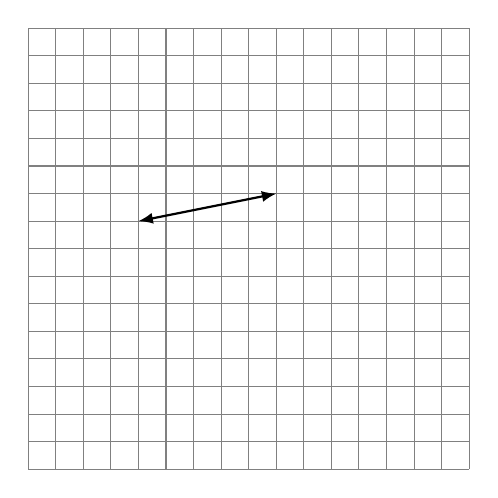
\begin{tikzpicture}[font=\tiny,scale=0.35]
   %\tikzstyle{every node}=[font=\small]
   \tkzInit[xmax=8,ymax=8,xmin=-8,ymin=-8]
   \tkzGrid
   \tkzAxeXY
   \draw[ thick,latex-latex] (-4,1) -- (1,2);% node[anchor=south west] {$a$}; % two points for drawing 2x+y=2
%  \tkzText[above](0,6.75){Desired Output}
  \end{tikzpicture}
\end{minipage}}%
\vspace{4cm}%
\item\adjustbox{valign=t}{\begin{minipage}{\linewidth}
What type of slope does the line in the graph have?\\

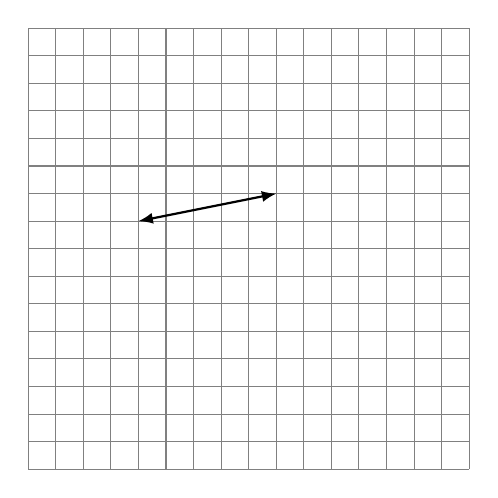
\begin{tikzpicture}[font=\tiny,scale=0.35]
   %\tikzstyle{every node}=[font=\small]
   \tkzInit[xmax=8,ymax=8,xmin=-8,ymin=-8]
   \tkzGrid
   \tkzAxeXY
   \draw[ thick,latex-latex] (-4,1) -- (1,2);% node[anchor=south west] {$a$}; % two points for drawing 2x+y=2
%  \tkzText[above](0,6.75){Desired Output}
  \end{tikzpicture}
\end{minipage}}%
\vspace{4cm}%
\item\adjustbox{valign=t}{\begin{minipage}{\linewidth}
What type of slope does the line in the graph have?\\

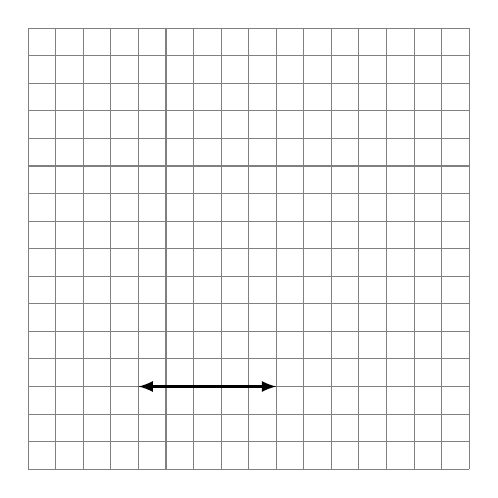
\begin{tikzpicture}[font=\tiny,scale=0.35]
   %\tikzstyle{every node}=[font=\small]
   \tkzInit[xmax=8,ymax=8,xmin=-8,ymin=-8]
   \tkzGrid
   \tkzAxeXY
   \draw[ thick,latex-latex] (-4,-5) -- (1,-5);% node[anchor=south west] {$a$}; % two points for drawing 2x+y=2
%  \tkzText[above](0,6.75){Desired Output}
  \end{tikzpicture}
\end{minipage}}%
\vspace{4cm}%
\item\adjustbox{valign=t}{\begin{minipage}{\linewidth}
What type of slope does the line in the graph have?\\

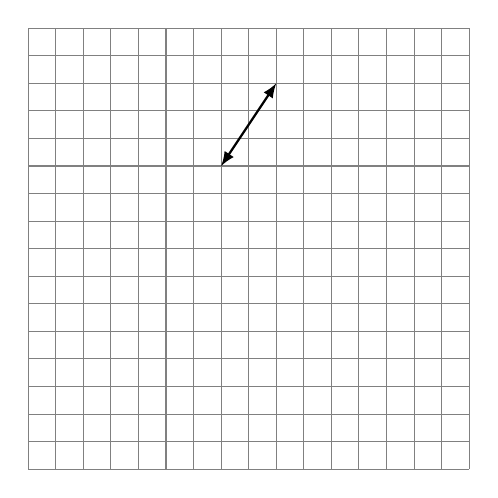
\begin{tikzpicture}[font=\tiny,scale=0.35]
   %\tikzstyle{every node}=[font=\small]
   \tkzInit[xmax=8,ymax=8,xmin=-8,ymin=-8]
   \tkzGrid
   \tkzAxeXY
   \draw[ thick,latex-latex] (-1,3) -- (1,6);% node[anchor=south west] {$a$}; % two points for drawing 2x+y=2
%  \tkzText[above](0,6.75){Desired Output}
  \end{tikzpicture}
\end{minipage}}%
\vspace{4cm}%
\item\adjustbox{valign=t}{\begin{minipage}{\linewidth}
What type of slope does the line in the graph have?\\

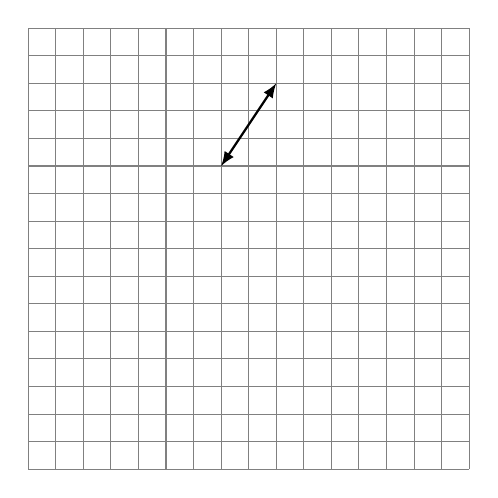
\begin{tikzpicture}[font=\tiny,scale=0.35]
   %\tikzstyle{every node}=[font=\small]
   \tkzInit[xmax=8,ymax=8,xmin=-8,ymin=-8]
   \tkzGrid
   \tkzAxeXY
   \draw[ thick,latex-latex] (-1,3) -- (1,6);% node[anchor=south west] {$a$}; % two points for drawing 2x+y=2
%  \tkzText[above](0,6.75){Desired Output}
  \end{tikzpicture}
\end{minipage}}%
\vspace{4cm}%
\item\adjustbox{valign=t}{\begin{minipage}{\linewidth}
What type of slope does the line in the graph have?\\

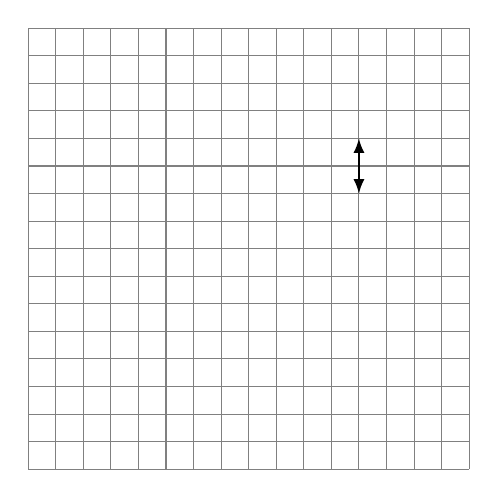
\begin{tikzpicture}[font=\tiny,scale=0.35]
   %\tikzstyle{every node}=[font=\small]
   \tkzInit[xmax=8,ymax=8,xmin=-8,ymin=-8]
   \tkzGrid
   \tkzAxeXY
   \draw[ thick,latex-latex] (4,4) -- (4,2);% node[anchor=south west] {$a$}; % two points for drawing 2x+y=2
%  \tkzText[above](0,6.75){Desired Output}
  \end{tikzpicture}
\end{minipage}}%
\vspace{4cm}%
\item\adjustbox{valign=t}{\begin{minipage}{\linewidth}
What type of slope does the line in the graph have?\\

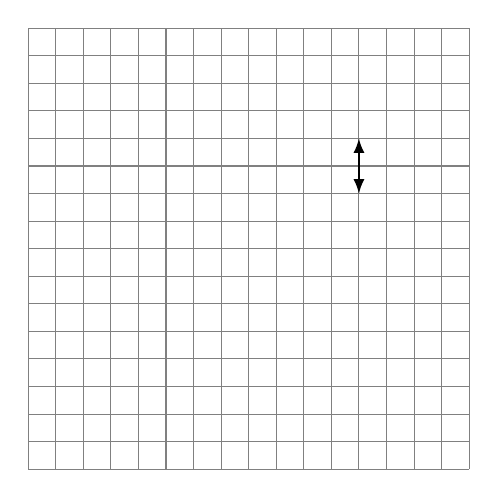
\begin{tikzpicture}[font=\tiny,scale=0.35]
   %\tikzstyle{every node}=[font=\small]
   \tkzInit[xmax=8,ymax=8,xmin=-8,ymin=-8]
   \tkzGrid
   \tkzAxeXY
   \draw[ thick,latex-latex] (4,4) -- (4,2);% node[anchor=south west] {$a$}; % two points for drawing 2x+y=2
%  \tkzText[above](0,6.75){Desired Output}
  \end{tikzpicture}
\end{minipage}}%
\vspace{4cm}%
\item\adjustbox{valign=t}{\begin{minipage}{\linewidth}
What type of slope does the line in the graph have?\\

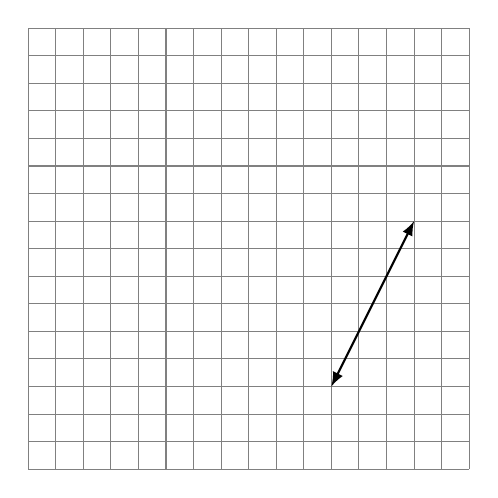
\begin{tikzpicture}[font=\tiny,scale=0.35]
   %\tikzstyle{every node}=[font=\small]
   \tkzInit[xmax=8,ymax=8,xmin=-8,ymin=-8]
   \tkzGrid
   \tkzAxeXY
   \draw[ thick,latex-latex] (3,-5) -- (6,1);% node[anchor=south west] {$a$}; % two points for drawing 2x+y=2
%  \tkzText[above](0,6.75){Desired Output}
  \end{tikzpicture}
\end{minipage}}%
\vspace{4cm}%
\item\adjustbox{valign=t}{\begin{minipage}{\linewidth}
What type of slope does the line in the graph have?\\

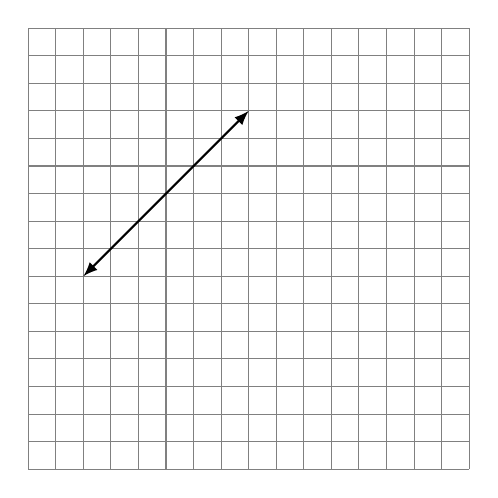
\begin{tikzpicture}[font=\tiny,scale=0.35]
   %\tikzstyle{every node}=[font=\small]
   \tkzInit[xmax=8,ymax=8,xmin=-8,ymin=-8]
   \tkzGrid
   \tkzAxeXY
   \draw[ thick,latex-latex] (-6,-1) -- (0,5);% node[anchor=south west] {$a$}; % two points for drawing 2x+y=2
%  \tkzText[above](0,6.75){Desired Output}
  \end{tikzpicture}
\end{minipage}}%
\vspace{4cm}%
\item\adjustbox{valign=t}{\begin{minipage}{\linewidth}
What type of slope does the line in the graph have?\\

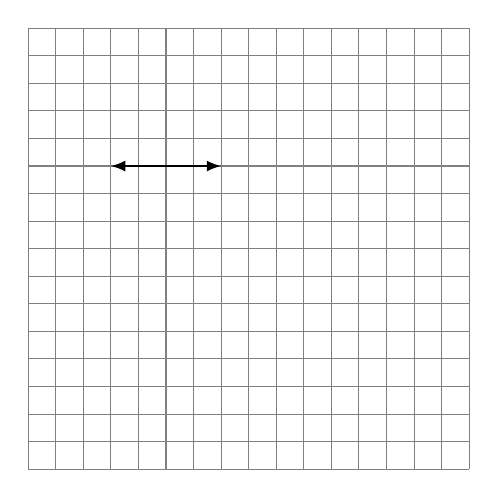
\begin{tikzpicture}[font=\tiny,scale=0.35]
   %\tikzstyle{every node}=[font=\small]
   \tkzInit[xmax=8,ymax=8,xmin=-8,ymin=-8]
   \tkzGrid
   \tkzAxeXY
   \draw[ thick,latex-latex] (-5,3) -- (-1,3);% node[anchor=south west] {$a$}; % two points for drawing 2x+y=2
%  \tkzText[above](0,6.75){Desired Output}
  \end{tikzpicture}
\end{minipage}}%
\vspace{4cm}%
\item\adjustbox{valign=t}{\begin{minipage}{\linewidth}
What type of slope does the line in the graph have?\\

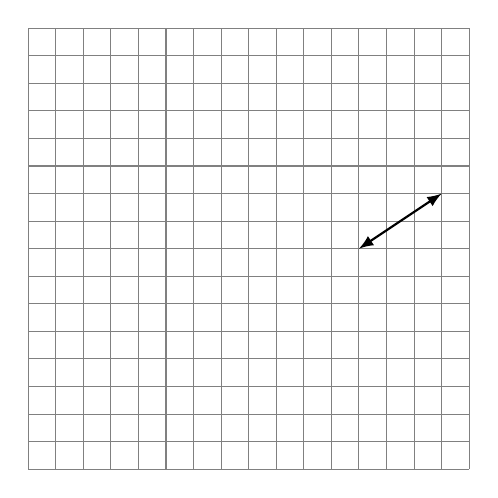
\begin{tikzpicture}[font=\tiny,scale=0.35]
   %\tikzstyle{every node}=[font=\small]
   \tkzInit[xmax=8,ymax=8,xmin=-8,ymin=-8]
   \tkzGrid
   \tkzAxeXY
   \draw[ thick,latex-latex] (4,0) -- (7,2);% node[anchor=south west] {$a$}; % two points for drawing 2x+y=2
%  \tkzText[above](0,6.75){Desired Output}
  \end{tikzpicture}
\end{minipage}}%
\vspace{4cm}%
\item\adjustbox{valign=t}{\begin{minipage}{\linewidth}
What type of slope does the line in the graph have?\\

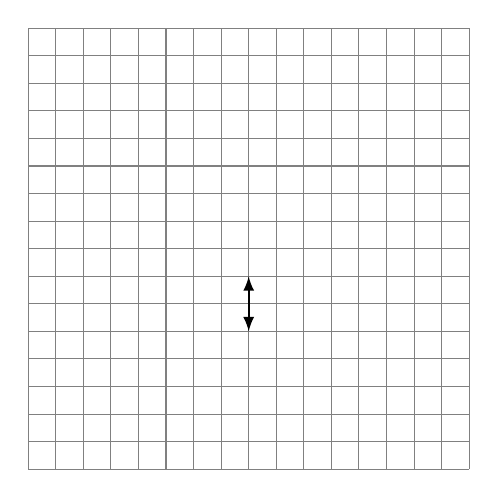
\begin{tikzpicture}[font=\tiny,scale=0.35]
   %\tikzstyle{every node}=[font=\small]
   \tkzInit[xmax=8,ymax=8,xmin=-8,ymin=-8]
   \tkzGrid
   \tkzAxeXY
   \draw[ thick,latex-latex] (0,-1) -- (0,-3);% node[anchor=south west] {$a$}; % two points for drawing 2x+y=2
%  \tkzText[above](0,6.75){Desired Output}
  \end{tikzpicture}
\end{minipage}}%
\vspace{4cm}%
\item\adjustbox{valign=t}{\begin{minipage}{\linewidth}
What type of slope does the line in the graph have?\\

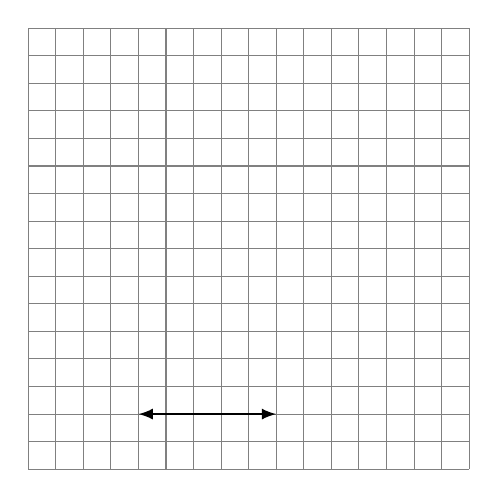
\begin{tikzpicture}[font=\tiny,scale=0.35]
   %\tikzstyle{every node}=[font=\small]
   \tkzInit[xmax=8,ymax=8,xmin=-8,ymin=-8]
   \tkzGrid
   \tkzAxeXY
   \draw[ thick,latex-latex] (-4,-6) -- (1,-6);% node[anchor=south west] {$a$}; % two points for drawing 2x+y=2
%  \tkzText[above](0,6.75){Desired Output}
  \end{tikzpicture}
\end{minipage}}%
\vspace{4cm}%
\item\adjustbox{valign=t}{\begin{minipage}{\linewidth}
What type of slope does the line in the graph have?\\

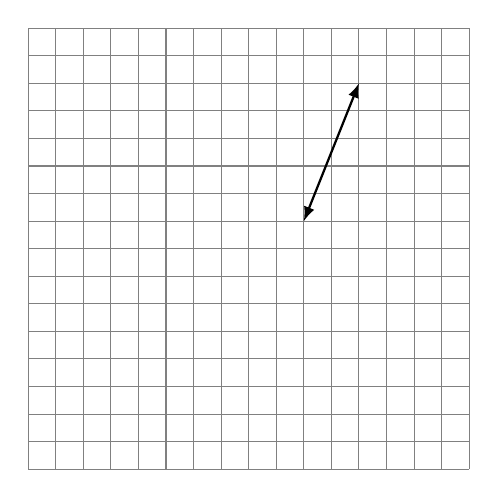
\begin{tikzpicture}[font=\tiny,scale=0.35]
   %\tikzstyle{every node}=[font=\small]
   \tkzInit[xmax=8,ymax=8,xmin=-8,ymin=-8]
   \tkzGrid
   \tkzAxeXY
   \draw[ thick,latex-latex] (2,1) -- (4,6);% node[anchor=south west] {$a$}; % two points for drawing 2x+y=2
%  \tkzText[above](0,6.75){Desired Output}
  \end{tikzpicture}
\end{minipage}}%
\vspace{4cm}%
\item\adjustbox{valign=t}{\begin{minipage}{\linewidth}
What type of slope does the line in the graph have?\\

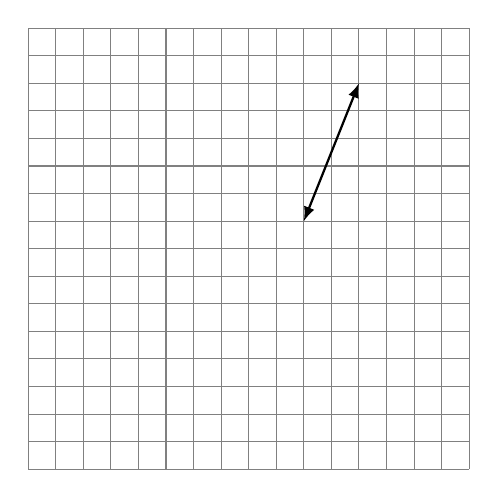
\begin{tikzpicture}[font=\tiny,scale=0.35]
   %\tikzstyle{every node}=[font=\small]
   \tkzInit[xmax=8,ymax=8,xmin=-8,ymin=-8]
   \tkzGrid
   \tkzAxeXY
   \draw[ thick,latex-latex] (2,1) -- (4,6);% node[anchor=south west] {$a$}; % two points for drawing 2x+y=2
%  \tkzText[above](0,6.75){Desired Output}
  \end{tikzpicture}
\end{minipage}}%
\vspace{4cm}%
\item\adjustbox{valign=t}{\begin{minipage}{\linewidth}
What type of slope does the line in the graph have?\\

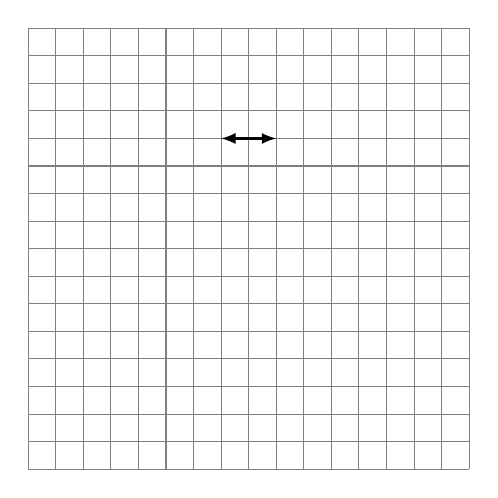
\begin{tikzpicture}[font=\tiny,scale=0.35]
   %\tikzstyle{every node}=[font=\small]
   \tkzInit[xmax=8,ymax=8,xmin=-8,ymin=-8]
   \tkzGrid
   \tkzAxeXY
   \draw[ thick,latex-latex] (-1,4) -- (1,4);% node[anchor=south west] {$a$}; % two points for drawing 2x+y=2
%  \tkzText[above](0,6.75){Desired Output}
  \end{tikzpicture}
\end{minipage}}%
\vspace{4cm}%
\item\adjustbox{valign=t}{\begin{minipage}{\linewidth}
What type of slope does the line in the graph have?\\

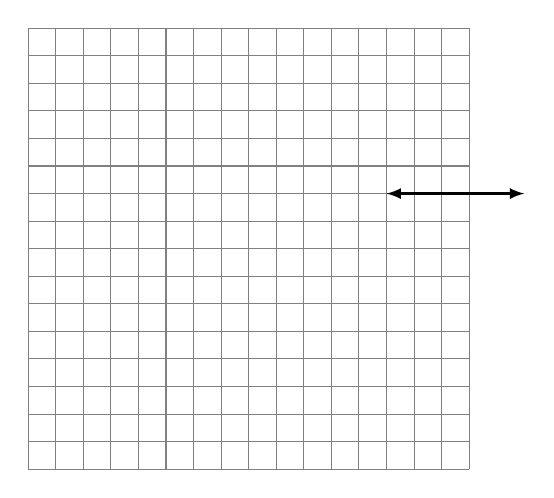
\begin{tikzpicture}[font=\tiny,scale=0.35]
   %\tikzstyle{every node}=[font=\small]
   \tkzInit[xmax=8,ymax=8,xmin=-8,ymin=-8]
   \tkzGrid
   \tkzAxeXY
   \draw[ thick,latex-latex] (5,2) -- (10,2);% node[anchor=south west] {$a$}; % two points for drawing 2x+y=2
%  \tkzText[above](0,6.75){Desired Output}
  \end{tikzpicture}
\end{minipage}}%
\vspace{4cm}%
\item\adjustbox{valign=t}{\begin{minipage}{\linewidth}
What type of slope does the line in the graph have?\\

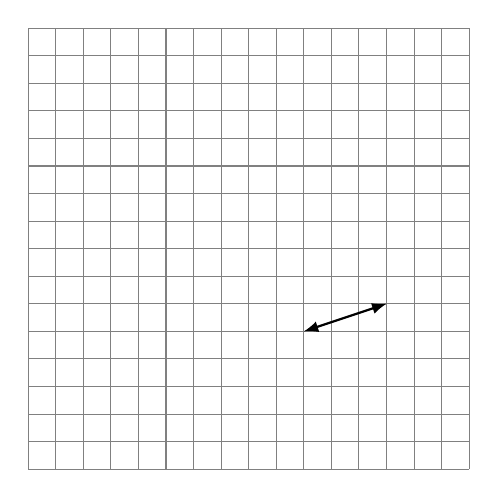
\begin{tikzpicture}[font=\tiny,scale=0.35]
   %\tikzstyle{every node}=[font=\small]
   \tkzInit[xmax=8,ymax=8,xmin=-8,ymin=-8]
   \tkzGrid
   \tkzAxeXY
   \draw[ thick,latex-latex] (2,-3) -- (5,-2);% node[anchor=south west] {$a$}; % two points for drawing 2x+y=2
%  \tkzText[above](0,6.75){Desired Output}
  \end{tikzpicture}
\end{minipage}}%
\vspace{4cm}%
\item\adjustbox{valign=t}{\begin{minipage}{\linewidth}
What type of slope does the line in the graph have?\\

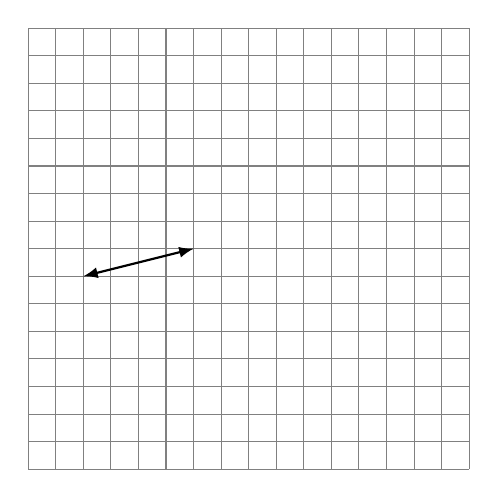
\begin{tikzpicture}[font=\tiny,scale=0.35]
   %\tikzstyle{every node}=[font=\small]
   \tkzInit[xmax=8,ymax=8,xmin=-8,ymin=-8]
   \tkzGrid
   \tkzAxeXY
   \draw[ thick,latex-latex] (-6,-1) -- (-2,0);% node[anchor=south west] {$a$}; % two points for drawing 2x+y=2
%  \tkzText[above](0,6.75){Desired Output}
  \end{tikzpicture}
\end{minipage}}%
\vspace{4cm}%
\item\adjustbox{valign=t}{\begin{minipage}{\linewidth}
What type of slope does the line in the graph have?\\

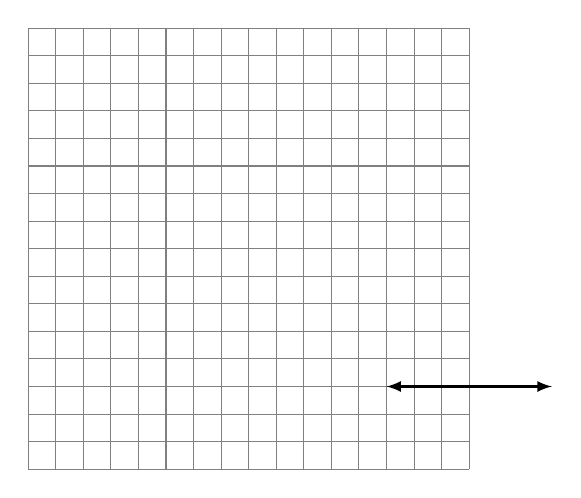
\begin{tikzpicture}[font=\tiny,scale=0.35]
   %\tikzstyle{every node}=[font=\small]
   \tkzInit[xmax=8,ymax=8,xmin=-8,ymin=-8]
   \tkzGrid
   \tkzAxeXY
   \draw[ thick,latex-latex] (5,-5) -- (11,-5);% node[anchor=south west] {$a$}; % two points for drawing 2x+y=2
%  \tkzText[above](0,6.75){Desired Output}
  \end{tikzpicture}
\end{minipage}}%
\vspace{4cm}%
\end{enumerate}

%
\end{multicols}%
\end{document}